\section{Software Testing}\label{sect:btesting}

This section introduces the software testing terminology, that is important in understanding the content of later sections. The first subsection describes the general terminology, while the second goes more into the specifics of ETL testing.

\subsection{Basic Testing}
In this subsection, we describe some core concepts relating to software testing. The information presented here is taken from the books \textit{Guide to Advanced Software Testing} by Hass\cite{Hass} and \textit{Software Testing Techniques} by Beizer\cite{Beizer}.

Testing is an integral part of the software development process. It is included in many different software process models. Hass defines testing as follows:
\begin{quotation} \textit{Testing gathers information about the quality of the object under test.}\end{quotation}
Knowing the quality of a piece of software allows an organization to evaluate, whether it upholds the requirements they set for it. If not, test results may guide an effort to increase quality.

Before tests can be executed, they must be designed. Design can be done from two different points of view: \emph{Functional} and \emph{Structural}. With functional, software is treated like a black box receiving input and computing output. Tests are designed to verify, whether the software conforms to specified behaviour. Structural involves designing tests based on the internal structure of the software.  A tester could for instance test how a piece of code logically branches during execution. The structural approach is often used, when testing individual components. Functional is likely to be used, when testing a set of integrated units or an entire system.

During the software testing process, a system is usually tested at different structural levels. During \emph{component testing}, each component of the system is tested in isolation. This usually requires the implementation of stubs and drivers. A stub simulates the code called by the component, while the driver simulates code, which the component is called by. The size of a component is defined by the organization, in which the code is tested. However, we can usually define a component as an aggregation of units. A Unit is the smallest testable part of a system, and it is itself defined to be a component. The testing of a single unit is often referred to as \emph{unit testing}. The difference between unit and component testing is that component testing considers not only units but also aggregated components. Through component testing we verify the quality of each component. Once verified we begin to integrate the components with each other. Here \emph{integration testing} may be performed. This type of test verifies the quality of the communication between the different components. After the system has been fully integrated, testers can perform \emph{system testing}. At this level of testing, we test the system as a whole. Thorough testing usually involves testing the software at each structural level in the order described. Structural testing is usually performed at the component and early integration level. Functional testing is used for both the later integration and system level.

As with any other process, testing is restricted by both time and resources available. These greatly affect the quality of testing performed, often called \emph{test coverage}. Because of this, testers are almost never able to perform exhaustive testing, where all combinations of input and preconditions are tested. Instead, testers select the most important areas to focus on during testing.

Tools are often used to assist in the testing process. An example is the testing framework, which often assist in the automatic execution of tests. A framework can execute a set of user-defined test cases, setting up and tearing down objects as needed. A test case is a well defined set of preconditions and input(s) given to a component. This is accompanied by a set of expected output(s) and postconditions. It either passes or fails, depending on whether the actual output and postconditions match expectations. The required test coverage is often acquired by designing a set of test cases. An advantage of frameworks is that testers can spend more time on test design. Yet, less time will be spent on how to implement tests. This leads to testing of a higher quality.

Another bonus of using a framework is that it allows for \emph{regression testing}. This becomes mostly relevant in the maintenance part of the software life cycle. During this time, new features may be added and bugs fixed. Testers want to ensure that such changes do not lead to regression, where software quality deteriorates. With a framework, regression testing is simple. Once a set of test cases have been set up, they can be run after a change has been made. This will help in gauging whether a regression has occurred.

\subsection{ETL Testing}

\begin{figure}
\centering
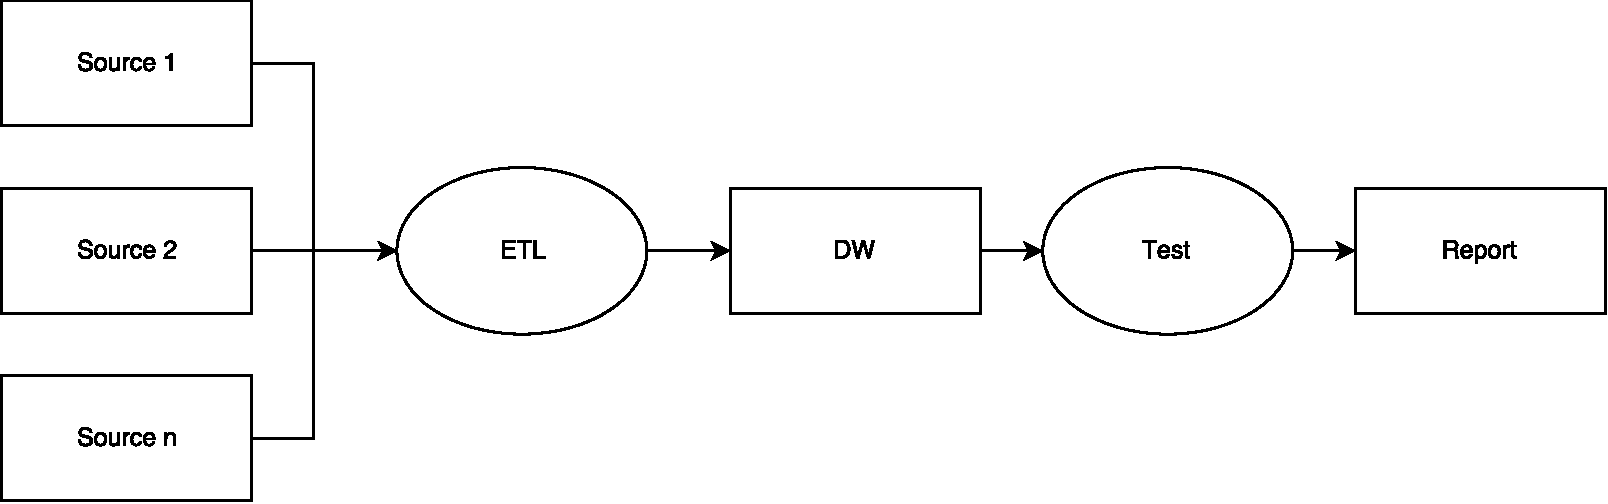
\includegraphics[width=0.5\textwidth]{figures/scenario.pdf}
\caption{An example of a source to target test used for ETL}
\label{fig:sourcetotarget}
\end{figure}

According to Rainardi in his book \textit{Building a Data Warehouse: With Examples in SQL Server}\cite{rainardi2007building} ETL testing assures that changes to sources are captured and propagated to the DW properly. Therefore, we can describe the core of ETL testing as being data-centric. Performance testing, which focuses on the speed of the transfer, is also relevant. However, for \FW{} we choose to focus on ETL testing as more of a data verification activity. Assertions are often used when testing an ETL system. They allow testers to assert about the program state. It can then be reported on whether the assertion held. As an example, a tester can assert that a variable has the value 5. Testers may make assertions at the component and early integration level. At these levels on-market unit testing tools may be used. As users of pygrametl are thought to be experts, we assert that they know how to perform this type of test. As such, developing a framework to assist in this process is not necessary.

Instead we choose to focus on testing at the system level, which is often called \emph{source to target} testing. An example is illustrated in \Cref{fig:sourcetotarget}. Here the ETL program under test populates a DW using a set of sources. Once the process has been finished, we test and report on whether assertions about the resulting DW have been met. Note that these assertions are different from those discussed earlier, as they function on a higher level of abstraction. They concern properties of the DW and its tables such as table length, functional dependency etc. This type of test is functional, as it does not test according to the internal structure of the system. Testing is performed according to system requirements. This method is also ideal for regression testing, as old assertions about DWs can simply be checked again.

What should \FW{} test during a source-to-target test? According to Rainardi \cite{rainardi2007building}, ETL testing is about ensuring that the data from sources ends up at the right locations of the DW. Thus data loss is a major concern. The checking of business rules is declared as a separate area of test. However, we argue that business rules are an important part of ETL testing. An ETL process should only load data into a DW, which conforms to agreed upon rules. Therefore we define the focal point of ETL testing to be both data loss and business rules. Both are touched upon in the remainder of this section.

\subsubsection{Data Loss}
Through an ETL process, data from sources are propagated into a DW. This new data contains information relevant to future business analysis. Yet, information may get lost during execution. Data loss can occur in any of the three sub parts of the ETL process. The wrong data may be extracted from the sources. Transformations may be faulty and produce incorrect results. Loss during load may happen through truncation. Truncation occurs, when the data type of a DW attribute can not store the amount of data necessary. This often results in data being cut to fit the data type. Any type of data loss results in a DW that does not contain required information. This may lead to faulty business analysis.

\subsubsection{Business Rules}
The term business rule is generally applied to any rule that states some constraint on the data stored in a DW. These may be unique to the business in question. For an airline, a rule could be that any passenger with over 10 flights in the last year should be registered to receive a special discount on snacks. Rules could also indicate attribute relationships such as hierarchies. These may state that a city must be located in a country.

Some more general business rules can be used to assert data integrity. Enforcing data integrity ensures the quality of data in a DW. Data integrity can be enforced using the following three types of rules:

\begin{itemize}
\item Entity integrity: Every table has a primary key, which is unique and not null for each row
\item Referential integrity: A foreign key has to refer to an existing primary key or be null
\item Domain integrity: An attribute should stay within its defined range of values
\end{itemize}

Data integrity is important, as it allows us to assert certain truths about our database. For instance, we know that each tuple is identifiable. Despite these advantages, DBMS' may not enforce them during loads. Loading data into a DW using an ETL usually involves a large amount of data, and access to the DW may be shut down temporarily. Enforcing data integrity during load is expensive. Therefore, a fast load often takes precedence over a safe load. If an ETL system is improperly designed, the DW ends up not having data integrity, which hinders its usefulness.